\section{Wyznaczanie całek wielokrotnych - kubatury}
\begin{frame}{Obszar prostokątny}
	  \begin{exampleblock}{}
        	\[
            	\iint_{R}f(x,\ y)dxdy \ \ 
                R=\{(x,\ y):a\leq x\leq b,\ c\leq y\leq d\}
            \]
            $ \ \ $a,b,c,d - stałe
            
            $\ \ $m. Simpsona: $\frac{b-a}{2n}; \ \  \frac{d-c}{2m}$
       \end{exampleblock}
\end{frame}
%%%%%%%%%%%%%%%%%%%%%
\begin{frame}
		\[
        	\iint_{R}f(x,\ y)dxdy= \int_{a}^{b}(\int_{c}^{d}f(x,\
            y)dx)dy=
        \]
        \[
        	\frac{k}{3}[\int_{a}^{b}f(x,\ 
            y_{0})dx
            +2\sum_{j=1}^{m-1}\int_{a}^{b}f(x,\ y_{2j})dx +  
        \]
        \[
        	4 \sum_{j=1}^{m}\int_{a}^{b}f(x,\ y_{2j-
            1})dx+\int_{a}^{b}f(x,\ y_{2m})dx]
        \]
        \[
        	-\frac{(d-c)k^{4}}
            {180}\int_{a}^{b}\frac{\partial^{4}f(x,\mu)}
            {\partial y^{4}}dx; \ \ \mu\in(c,\ d)
        \]
        $\newline$
      	i dla $\forall$ z całek: zł. wzór Simpsona z 
        $x_{i}=a+ih, \ \ i=0, 1, 2, . . . , 2n$
\end{frame}
%%%%%%%%%%%%%%%%%%%%%%
\begin{frame}
	\begin{block}{Zadanie 1.}
        	Rysunek, wzrór całkowy, błąd
       \end{block}
	$\newline$
   \begin{block}{Zadanie 2.}
        	Złożoność obliczeniowa; to samo dla m. Gaussa
   \end{block}
\end{frame}
%%%%%%%%%%%%%%%%%%%%%%%%%%%%%
\begin{frame}{Obszar normalny względem OX}
	    \begin{figure}[h]
			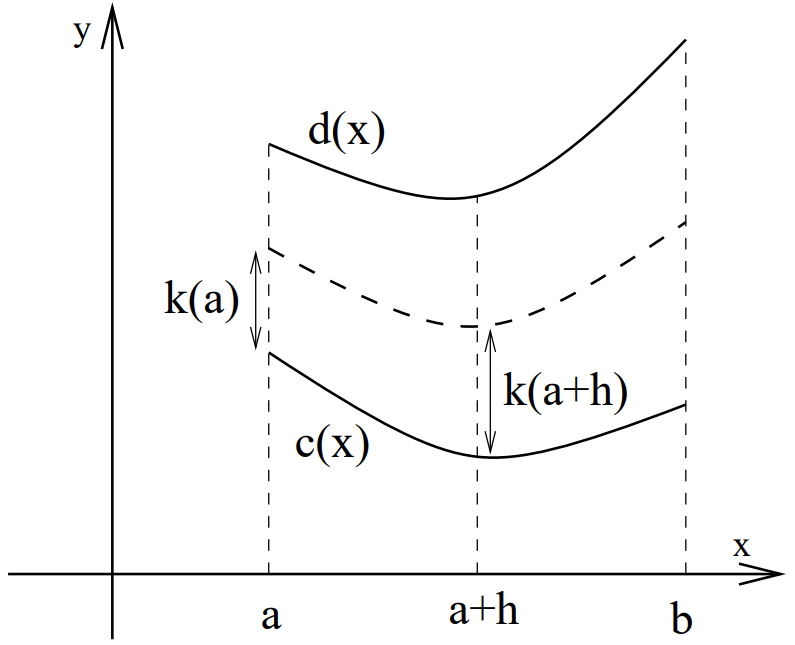
\includegraphics[width=.55\linewidth]{img/6/6_01}
		\end{figure}
        \[
        	\int_{a}^{b}\int_{c(x)}^{d(x)}f(x,\ y)dxdy;
        \]
        wzdłuż x: $h=\frac{b-a}{2}$
        $\newline$
        wzdłuż y: $k(x)=\frac{d(x)-c(x)}{2}$
\end{frame}
%%%%%%%%%%%%%%%%%%%%%%%%%%%%%%%%
\begin{frame}
	\[
    	I\approx\int_{a}^{b}\{\ \frac{k(x)}{3}[f(x,\ 
        c(x))+4f(x,\ c(x)+k(x))+f(x,\ d(x))]\}dx\approx\ldots
    \]
    \begin{block}{Zadanie}
        	Powyższy wzór - dokładniej
            $\newline$
            każda z całek - wzór Simpsona
   \end{block}
\end{frame}
%%%%%%%%%%%%%%%%%%%%%%%%%%%%%%%
\begin{frame}{Obszar regularny}
	\begin{block}{}
      \begin{itemize}
      \item całkowanie zewnętrzne - wewnętrzne
      \item dla ustalonego y - właściwy dobór x
      \item nie stosujemy regularnej siatki prostokątnej
      \end{itemize}
	\end{block}
\end{frame}
%%%%%%%%%%%%%%%%%%%%%%%%%%%%%%%%%%
\begin{frame}{Uwagi ogólne}
	\begin{enumerate}
	\item całki n-D nie są proste!
    \item złożoność obliczeniowa:
    	\begin{itemize}
    		\item 1-D $\rightarrow$ 30 obliczeń funkcji
            \item 3-D $\rightarrow$ $30^3 = 27000$ obliczeń!
    	\end{itemize}
    \item obszar całkowania:
    	\begin{itemize}
    		\item 1-D $\rightarrow$ zdefiniowany przez 2 punkty 
    	\end{itemize}
    \item n-D $\rightarrow$ $(n-1)D$ granica $\rightarrow$ skomplikowana!
	\end{enumerate}
\end{frame}
%%%%%%%%%%%%%%%%%%%%%%%%%%%%%%%%%%
\begin{frame}
	   \begin{figure}[h]
			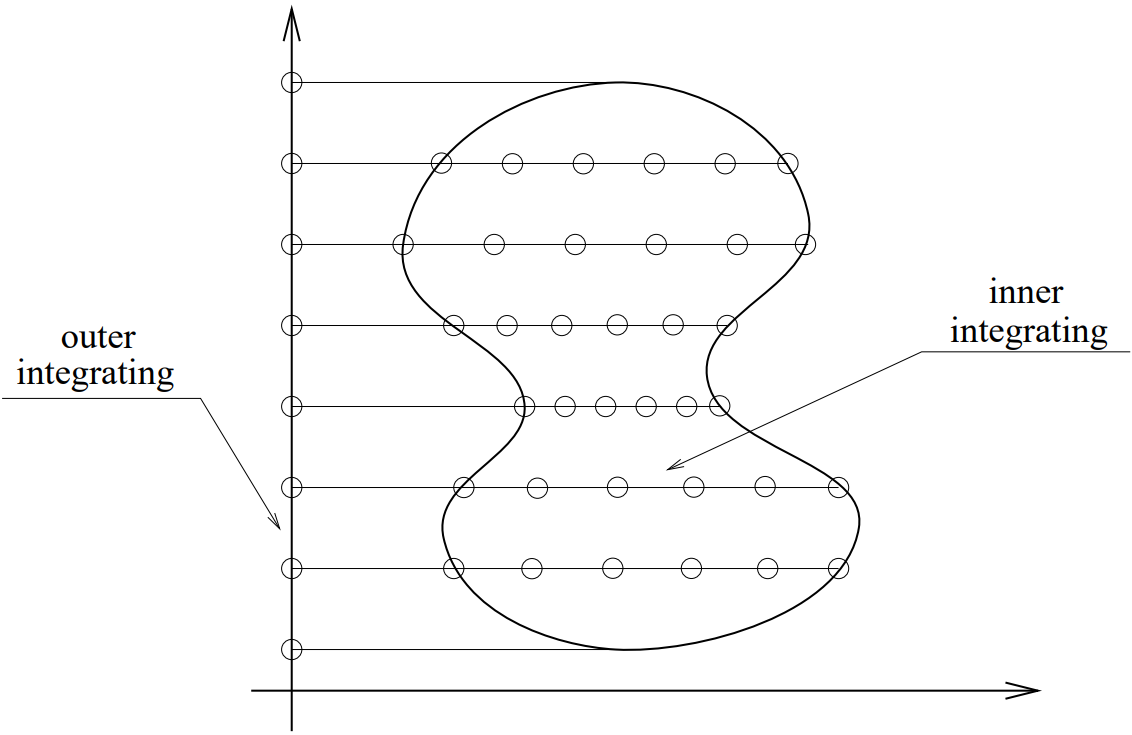
\includegraphics[width=.85\linewidth]{img/6/6_02}
		\end{figure}
\end{frame}
%%%%%%%%%%%%%%%%%%%%%%%%%%%%%%%%%
\begin{frame}
	\begin{large}
		\textbf{Podejście:}
	\end{large}
	\begin{itemize}
	\item analityczme (co się da!)
    \item wykorzystać symetrie
    \item metoda całkowania zależna od przebiegu funkcji w poszczególnych obszarach
    \item stosowanie metod Monte-Carlo
	\end{itemize}
\end{frame}
%%%%%%%%%%%%%%%%%%%%%%%%%%%%%%%%
\begin{frame}
	Całkę n-krotną można wyrazić wzorem przybliżonym:
    \[
     \int \ldots \int_{A} w(x_{1}, \ldots , x_{n})
     f(x_{1}, \ldots , x_{n})dx_{1},\ldots , dx_{n}
     \approx
     \sum_{i=1}^{n}H_{i}f(x_{1}^{(i)}, \ldots , x_{n}^{(i)})
    \]
    $A$ - obszar, $\ \ $ $w(x_{1}, \ldots , x_{n})$ - waga
    $\newline$
    $H_{i}, x^{(i)}_{j}$ - dobrane tak, by wzór był dokładny dla 
    wielomianu stopnia $\leq d$
    \begin{block}{Zadanie}
        	Wyznaczanie całek niewłaściwych
   \end{block}
\end{frame}




































